\documentclass{acm_proc_article-sp}

%packages
\usepackage{epstopdf}
\usepackage{hyperref}
\usepackage{tikz}
\usepackage{algpseudocode}
\usepackage{algorithm}
\usepackage{cleveref}
\usepackage{todonotes}
\usepackage{cite}
\usepackage{pgfplots}
\usepackage{siunitx}
\usepackage{tikz}
\usetikzlibrary{arrows,automata}
\usepackage{siunitx}
 
\DeclareSIUnit\Wh{Wh}

\begin{document}

\title{Fastest-Path Algorithm for Electrical Vehicles}

\numberofauthors{4} 
\author{
% 1st. author
		\alignauthor A. B. Eriksen\\
       \affaddr{Institute of Computer Science}\\
       \affaddr{Aalborg University}\\
       \email{aeriks11@student.aau.dk}
% 2nd. author
		\alignauthor M. A. Madsen\\
       \affaddr{Institute of Computer Science}\\
       \affaddr{Aalborg University}\\
       \email{mman10@student.aau.dk}
\and
% 3rd. author
		\alignauthor
		M. M. Andersen\\
       \affaddr{Institute of Computer Science}\\
       \affaddr{Aalborg University}\\
       \email{mama11@student.aau.dk}
% 4th. author
		\alignauthor
		S. B. Jensen\\
       \affaddr{Institute of Computer Science}\\
       \affaddr{Aalborg University}\\
       \email{sbje11@student.aau.dk}}
\date{30 July 2014}
\maketitle

\begin{abstract}
We describe a greedy heuristic algorithm for finding the fastest path, between two points in a
large road network graph, for electric vehicles (EVs). We further introduce a linear programming 
approach, which could be combined with the greedy heuristic algorithm and likely improve fastest path 
finding abilities at the cost of run time performance. Unlike many of today's GPS systems, the greedy heuristic 
algorithm takes both the drive time and the recharge time into account. Since the recharging possibilities for 
electric vehicles are still limited on Danish roads and the recharging process takes a long time compared to refuelling 
times of regular gasoline cars, this is necessary in order to give the electric vehicles users a 
useful route plan.\\

We compared the performance of the greedy heuristic algorithm with a naive algorithm on road
networks extracted from OpenStreetMap (OSM). We modified the OSM road network, so it contained Danish speed limits
and charge stations at variable positions and with variable charge rates. We compared the performance of the algorithms 
with four different parameters: the density of charge stations in the road network, the charge rates of the charge stations 
in the road network, the size of the road network measured in distance and the complexity of the road network measured 
in number of nodes. HOW DID IT PERFORM?!      

\end{abstract}

\keywords{Shortest-path algorithm with resource constraints, Electrical vehicles, Road-network, Route planing} % NOT required for Proceedings

\section{Introduction}

As the adoption rate of electric vehicles increases \cite{Henry2013}, the need for a better and more complex route planing solution appears. Electric vehicles generally have a shorter range as well as a significantly slower recharge time, compared to traditional gasoline cars. As the recharge time have become a significant factor in the total travel time, the time spend recharging should be taken into account by a route planning system, to accommodate for an otherwise large margin of error. Time spend recharging batteries is inherently variable, as the charge rate is affected by both the charge station's charge rate as well as the battery's current charge. When planning a fastest-path route for an electric vehicle, it is therefore paramount to be able to incorporate charge station's charge rates and electric vehicle's battery.\\

Another important aspect is the electric vehicle's energy consumption rate. With the now significant time spend recharging, a high consumption rate while driving, can in turn result in a slow route due to increased charging time. The consumption rate of a electric vehicles generally increases polynomially with speed, primarily due to aerodynamics \footnote{Aerodynamic losses are important especially at high speeds. The force of air friction is given by equation: $F = \frac{1}{2} \rho V^2 A C_d$, where $\rho$ is the air density, $A$ is the frontal area of the vehicle, $C_d$ is the drag coefficient and $V$ is the speed}, so the consumption rate should also be taken into account by the route planning system. Furthermore the rate of charging of the battery in electrical vehicles is a polynomial function, i.e. the battery is charged substantially faster from 0\% to 80\% compared with 80\% to 100\%. We will ignore this fact, as this is arguably not a substantial problem. One could simply linearize the function for the battery.\\

It should be clear that no traditional shortest path algorithm is able to accommodate for the variables and relationships between the speed, the consumption rate, the charge rate and the current charge of the electric vehicle. In this article, we present a Greedy-heuristic algorithm for solving the problem of optimising a route plan for electric vehicles. We also introduce a linear programming approach which could be combined with the Greedy-heuristic algorithm. The algorithm with and without linear programming are analysed on their running time and reliability.







\section{Notation}
In this section we will briefly explain the mathematical notation and model used in the paper. The graph representation consists of edges which represent road segment and vertices which represent either charge stations or road intersections. We define a \textbf{road network} as an ordered pair \(G=(V,E)\) comprising of a set $V$ of vertices together with a set $E$ of edges. Where $V$ is a finite set and $E$ is a binary relation on $V$. We further define the following functions:
\[ D(e)\rightarrow d \] 
\[ V_{max}(e)\rightarrow v \] 
These total functions respectively return a distance or a velocity limit, with and edge $e$ as argument.

We define a path of length k from a vertex $u$ to a vertex $u'$ in a graph as a sequence of vertices $\langle v_0,v_1,v_2,\dots,v_k \rangle$ such that $u=v_0$, $u'=v_k$ and $(v_{i}),v_{i+1})\in E$ for $i=1,2,\dots ,k-1$.

Each vertex is defined as a \textit{charge station}, described by the following total function:
\[CH(v)\rightarrow c\]
A road intersection is simply a vertex with charge rate $c = 0\si{\W}$, while a charge station is a vertex where $c > 0$. An electrical vehicle is specified by two parameters: It's battery capacity given in $\si{\Wh}$, and the consumption rate of the vehicle in $\si{\Wh\per\metre}$. The consumption rate is given by the following function:

\[CS(v)=av^2+bv+c\]
% \[ 4,60272*10^{-5}*v^2+6,59187*10^{-4}*v+0,173117 \] tesla

where $v$ is the speed of the vehicle. The constants $a$,$b$,$c$ are dependent on the the specific instance of the vehicle  

The charge of the battery given in $\si{\Wh}$ is a function of the start charge, the energy consumed and the energy charged. However we will abstract away from this, as this is uselessly complicated to write, and just denote $B_{cur}$ as the current battery charge.

\subsection{Shorter Not Equal Faster}

A shorter path does not necessarily mean a faster path for electrical vehicles. 
This is partly due to the fact that an electrical vehicles uses polynomially more energy as its speed increases but also due to the fact that charge times on charge stations
varies a lot. Driving a longer path with a fast charge station on can therefore turn out to
be a faster choice than driving a shorter path with a slow charge station on. This is illustrated 
in Figure~\Cref{fig:simpleroad-network}. In the example we assume our car has a battery capacity of 100 kWh and a energy-usages of
0,4 kWh/km. Path 1 consist of two edges with distance = 250 km and speed limit = 100 km/t
and a charge station with a charge speed of 200 kWh/t. Path 2 consist of two edges with
distance 200 km and speed limit 100 km/t and a charge station with a charge speed of 30 kWh/t.
The total time of each path:
				
\textbf{Path 1:} \text{route time} = ((250km + 250km) / 100km/h) + (100kWh / 200kWh/h) = 5,5h
				
\textbf{Path 2:} \text{route time} = ((200 km + 200 km) / 100 km/h) + (60 kWh / 30 kWh/h) = 6 h

\subsection{Optimization algorithm}
The first solution model we propose for finding the fastest path between two points in a road network is based on a linear programming approach. 
The algorithm consists of continuous pruning of paths in the road network, until we end up with a single path which is the optimal one. Initially, we pick a random path from $s$ to $t$, called $p$, and solve it optimally, which returns time $T_p$. For every other paths, $p'_i$, from $s$ to $t$ in the road network, we calculate the time it takes to pass it at maximum speed and without charging, which returns time $T_{p'_{i}}$. If $T_p \leq T_{p'_{i}}$ for any $p'_{i}$, we simply ignore it and all it's sub-paths. We can do this, since the optimally time spend driving $p'_i$ will be either greater than or equal to $T_{p'_{i}}$. If we find a path which can be driven faster than $T_p$ we update $p$ and $T_{p'}$. Determining how a path is optimally solved is described in section \ref{sec:optimizingwithLP}. But the overall algorithm for finding the fastest path looks as follows:

\begin{algorithmic}
\Function{fastestPath}{$G,s,t$}
    \State $p \gets$ initial\_path($G,s,t$) 
    \State $T_p \gets$ solve\_optimally($p$)
    \State $potential\_paths \gets$ get\_paths($G,s,t,T_p$)
    \Repeat 
    	\State $T_{p_1} \gets$ solve\_optimally(potential\_paths[1])
    	\If{$T_{p_1} < T_p$} 
    		\State $T_p \gets T_{p_1}$
    		\State $p \gets potential\_paths[1]$ 
    	\EndIf  
    	\State $paths.remove(potential\_paths[1])$
    	\ForAll{$p \in potential\_paths$} 
    		\If{$T_p \leq p.min$}
    			\State $potential\_paths.remove(p)$
    		\EndIf
    	\EndFor
    \Until{$potential\_paths.size = 0$}
    \State \Return $(p, T_p)$
\EndFunction
\end{algorithmic}

$initial\_path(G,s,t)$ returns a randomly chosen path, $p$ which is solved optimally by $solve\_optimally(p)$. $get\_paths(G,s,t,T_p)$ returns a sorted list of paths in $G$ between $s$ and $t$ with a max travelling time of $T_p$.

\subsection{Optimization problem}
We now describe how we calculate the speed to drive at and the amount of energy to charge at which charge stations, in order to pass a path optimally in terms of time. The paths the optimization problem is intended to solve are modelled in the following way: \\
\begin{figure}[h!]
\centering
    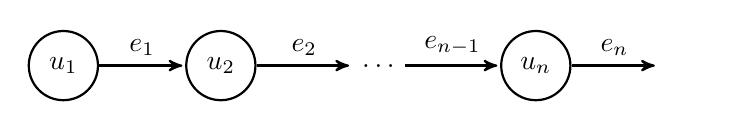
\begin{tikzpicture}[shorten >=1pt,node distance=2cm,>=stealth',thick]
        \node[state] (1) {$u_1$};
        \node[state] (2) [right of=1] {$u_2$};
        \node[] (dots) [right of=2] {$\dots$};
        \node[state] (n) [right of=dots] {$u_n$};
        \node[state,draw=none] (d1) [right of=n] {};
        \draw [->] (1) to[right] node[auto] {$e_1$} (2);
        \draw [->] (2) to[right] node[auto] {$e_2$} (dots);
        \draw [->] (dots) to[right] node[auto] {$e_{n-1}$} (n);
        \draw [->] (n) to[right] node[auto] {$e_n$} (d1);
    \end{tikzpicture}
    \caption{Example of a path consisting of $n$ edges} \label{fig:pathexample}
\end{figure} \\

The objective of the optimization problem is to minimize the time spend driving 
and the time spend charging for the entire path. The optimization problem can be expressed as follows:

\begin{equation}
	\begin{aligned} & \underset{v_{e_{1}} \dots v_{e_{n}}}, charge\_time(u_1 \dots u_n)}}
	{\text{minimize:}}
	& & \sum_{i=1}^{n} \frac{D(e_i)}{v(e_i)} + charge\_time(u_i) \\
	\end{aligned}
\end{equation}\label{eq:objfunction}

The problem needs to be solved accordingly to a set of constraints, the constraints can be formulated at follows: \\
On all edges the speed of the electrical vehicle must be within the speed limits. $v(e_i)$ is the speed on edge $e_i$. $v_{min}(e_i)$ and $v_{max}(e_i)$ is the minimum and maximum speed limit. So we have that $v_{min}(e_i) <= v(e_i) <= v_{max}(e_i)$ for all .
 
\begin{equation}
v_{min}(e_i) <= v(e_i) <= v_{max}(e_i) \text{for} i = 1..n  
\end{equation}

The battery level of the EV, $B_{cur}$, needs to be between $0$ and the max capacity of the vehicles battery. This constraint is split up in two constraints, one ensuring that the EV will have enough energy to drive each edge and one ensuring that the EV can not over charge at any charging station. $C_R(v)$ is the the energy consumption function of the EV.

\begin{equation}
\begin{aligned}
& \forall_{i \in 1 \dots n}: \; 0 \leq \sum_{j=1}^{i} \; chargerate_j*charge_j - \\
&  \sum_{j=1}^{i} \; distance_j*C_R(v_j) \leq maxbattery \\
 \end{aligned}
\end{equation}

\begin{equation}
\begin{aligned}
& \forall_{i \in 1 \dots n-1}: \; 0 \leq \sum_{j=i}^{i+1} chargerate_j*charge_j - \\
&   distance_i*C_R(v_i) \leq maxbattery \\
 \end{aligned}
\end{equation}

It should also not be possible for the EV to spend a negative amount of time at a charge station.

\begin{equation}
\forall_{i \in 1 \dots n}: \; 0 \leq charge_i 
\end{equation}

This optimization problem is almost a linear programming problem. We to however suffer from a non-linear constraint $distance_i*C_R(v_i)$ since the consumption rate $C_R(v)$ of the EV is not linear. The function can however be estimated using linearization. Using linearization we end up with the following linear programming problem.  
 
minimizing the sum of time spend driving and the sum of time spend charging. 

\begin{equation}
\begin{aligned}
 & \underset{speed_{1 \dots n},charge_{1 \dots n}}
{\text{minimize}}
& & \sum_{i=1}^{n} \frac{Distance_i}{speed_i} + charge_i \\
\end{aligned}
\end{equation}\label{eq:objfunction}

subject to: 
\begin{equation}
\forall_{i\in1 \dots n }:\; \sum_{j=1}^{m} Selectedlines[i,j] = 1
\end{equation}

\begin{equation}
\forall_{i\in1 \dots n, j \in 1 \dots m}: \; \;0\leq Selectedlines[i,j] \leq 1
\end{equation}

\begin{equation}
\forall_{i\in1 \dots n, j \in 1 \dots m}:\; speed[i,j] \le Selectedlines[i,j] * Points1[i,j]
\end{equation}

\begin{equation}
\forall_{i\in1 \dots n, j \in 1 \dots m}:\; speed[i,j] \ge Selectedlines[i,j] * Points2[i,j]
\end{equation}

\begin{equation}
\begin{split}
\forall_{k\in1 \dots n}\;:\;0 \le\sum_{i=1}^{k}chargerate[i]*charge[i]\\
-\sum_{i=1}^{k} distance[i](\sum_{j=1}^{m} LinesA[i,j]*speed[i,j]\\
+\sum_{j=1}^{m} Selectedlines[i,j]*LinesB[i,j]) \le maxbattery\;capacity
\end{split}
\end{equation}



\subsection{Optimizing with heuristics}


\section{Experiments}
\label{sec:experiments}
Now we present the experiments of the Greedy Heuristic Algorithm. It was concluded that the practical usage of the linear programming solution was not plausible in our experiments, after several implementations using an existing solver. Additionally, there will be a runtime complexity test of the algorithms.

We have constructed four experiments, to figure out what implication the adjusting of these parameters will have on the Greedy Heuristic Algorithm. The four parameters being experimented on are:
\begin{itemize}
     \item Route driving distance
     \item Charge rate of charge stations
     \item Consumption rate of EVs
     \item Density of charge stations
 \end{itemize} 

\todo[inline]{insert default values}


\subsection{Road network dataset} 
\label{sub:setup}
To facilitate the experiments, we've had to find a real world road network dataset which contains road distances, speed limits and charge stations of varying charge rates. Such a dataset does not openly exist to our knowledge. Instead we have used OpenStreetMaps which is an open-source collection of map data. One can read more about OSM at \url{http://www.openstreetmap.org/about}. OSM has a concept of ways and vertices. Ways represent geographical planar objects e.g. roads, cycleways, foot ways etc. A vertex is a geographical point consisting of a latitude and longitude coordinate. A way is constituted of a set of vertices and some tags which describe meta-information about the way, such as the name of the way and what type of way it is e.g. a road, cycleway, foot way  etc. From this information we can derive that if way $e_1$ and $e_2$ intersect in vertex $u$, they will share the vertex $u$. A vertex is referred to as either a road intersection or as a charge station if the vertex has been assigned a charge rate.\\

The ways and vertices can easily be converted into a, for us, useful road network structure for experimenting. This is done, by simply filtering away all types of ways accept roads and use these as edges in the road network. To get a notion of speed limits on edges, we derive general speed limits from the type of the roads. OSM carries such information as whether the road is a motorway, residential way, tertiary way etc. The speed limits are set according to Danish speed limits. For vertices, we are only interested in the ones which correspond to intersections between two roads. All other vertices in the road network are ignored. To get a notion of charge rate on the vertices we have implemented a method which distributes random charge rates on randomly selected vertices in the road network.\\

We have used the drivable part of Denmark as a baseline for the experiments. The dataset features:
\begin{itemize}
    \item 483407 vertices
    \item 543482 edges
\end{itemize}

\subsection{Naive algorithm}
\label{sub:naivealgorithm}
We have formulated a naive algorithm for performance comparison with our greedy-heuristic algorithm. The naive algorithm should simulate the way a naive electric vehicle driver would choose to travel through a road network. The naive algorithm works the following way: It greedily chooses the fastest roads in terms of distance over speed. Whenever the battery reaches 40 \% battery capacity, it starts searching for nearby charge stations in the radius allowed by the 40 \% battery capacity given the vehicles consumption rate. If no charge stations are available with 40 \% battery capacity, the path from $s$ to $t$ is not solvable for the naive algorithm. If, on the other hand, one or more charge stations are reachable, the algorithm will choose the closest one and charge to 100 \% battery capacity or to the battery capacity needed in order to reach $t$. After charging, the algorithm will resume greedily choosing the fastest roads from the charge station to $t$, in terms of distance over speed.

\subsection{Experiment: Complexity of Road Network}

We compared the run-time of the Greedy-heuristic algorithm to the naive algorithm with the complexity of the road network as changing parameter. The
complexity is measured in the number of vertices on the road network. The more vertices on the road network, the more vertices the two algorithms has 
to visit before they are able to find a fastest path. The set-up of the experiment: distance to drive was 100 km, the minimum distance between 
charge stations was 20 km. The initial number of vertices in the road network: 450000 vertices. The number of vertices is then counted down with 10000 for each iteration of the test. The resulting graph is illustrated in (REF!).

\subsection{Experiment: Density of Charge Stations}

We compared the performance of the Greedy-heuristic algorithm to the naive algorithm with the density of charge stations as changing parameter. The
density of charge stations are measured in the minimum distance between two charge stations. Initially, the minimum distance is set to 5 km which generates 3029 charge stations in Denmark. Table \ref{table:chargedensity} shows the number of charge stations according to the minimum distance between charge stations in the road network.

\begin{table}[!htb]
\centering
		\begin{tabular}{ p{1.85cm} p{0.67cm} p{0.63cm} p{0.63cm} p{0.63cm} p{0.63cm} p{0.63cm} } \hline
		Radius (km): & 5 & 10 & 20 & 30 & 40 & 50 \\ \hline
		Stations: & 3029 & 827 & 326 & 117 & 76 & 49 \\ \hline 
		\end{tabular}
		\caption{number of charge stations corresponding to the minimum distance between two charge stations}
	\label{table:chargedensity}
	\end{table}

The set-up of the experiment: the distance to drive was set to 200 km, the complexity of the road network was 483398 vertices, which is the number of vertices in Denmark. The charge rates of the charge stations are evenly distributed with rates between $10 \si{\kW}$ and $100 \si{\kW}$. The resulting graph is illustrated in (REF!).

\subsection{Experiment: Charge Rate on Charge Stations}

We compared the performance of the Greedy-heuristic algorithm to the naive algorithm with the charge rate of charge stations as changing parameter. The minimum distance between charge stations was set to 30 km, the distance to drive was set to 200 km. The initial charge rates in the road network were evenly distributed between $10 \si{\kW}$ and $100 \si{\kW}$. For each iteration all charge rates are scaled with a constant factor resulting in worse of better charge rates on all charge stations. The resulting graph of the experiment is seen in (REF!). On the x-axis is displayed the average charge rate of the charge stations on the road network. On the y-axis is displayed the time it takes to pass a path of length 200 km. 

\subsection{Experiment: Size of Road Network}



\subsection{Citations}

\section{Conclusion}
\label{sec:conclusion}
As the adoption rate of EVs increases time-optimised route planning systems for electrical vehicles will become increasingly important. 
We showed that a route planning system for EVs should take charging stations and charging rates into account, since the time spend 
charging an EV with today's standards is still relatively long. 

The problem of finding a route plan for an EV can be modelled as an optimisation problem. We implemented a greedy heuristic algorithm that used greedy choices and heuristics about the EV and the road network to find time-optimised paths. We ran several experiments on a real world road network and compared the performance with a naive algorithm that simulated the pattern of a naive electric vehicle driver. The experiments showed that the greedy heuristic algorithm both finds better paths and better charging plans than the naive algorithm. The worst-case time complexity of the greedy heuristic algorithm is $O(|V||E|+|V^2|\log|V|)$

We further implemented a linear programming solution using GNU Linear Programming Kit but found that solving every simple path in a graph with the size of a real world road network, is simply too expensive to compute within reasonable time. We compared the path time outputted by the greedy heuristic algorithm to the path time of the linear programming solution when run on the same path. \todo[inline]{How good are the paths found relative to the linear programming solution?}
  

%ACKNOWLEDGMENTS are optional
%%ACKNOWLEDGMENTS are optional
\section{Acknowledgements}
This section is optional; it is a location for you
to acknowledge grants, funding, editing assistance and
what have you.  In the present case, for example, the
authors would like to thank Gerald Murray of ACM for
his help in codifying this \textit{Author's Guide}
and the \textbf{.cls} and \textbf{.tex} files that it describes.	

\subsection{References}
Generated by bibtex from your ~.bib file.  Run latex,
then bibtex, then latex twice (to resolve references)
to create the ~.bbl file.  Insert that ~.bbl file into
the .tex source file and comment out
the command \texttt{{\char'134}thebibliography}.
% This next section command marks the start of
% Appendix B, and does not continue the present hierarchy

\end{document}
